%%%%%%%%%%%%%%%%%%%%%%%%%%%%%%%%%%%%%%%%%
% The Legrand Orange Book
% LaTeX Template
% Version 2.1.1 (14/2/16)
%
% This template has been downloaded from:
% http://www.LaTeXTemplates.com
%
% Original author:
% Mathias Legrand (legrand.mathias@gmail.com) with modifications by:
% Vel (vel@latextemplates.com)
%
% License:
% CC BY-NC-SA 3.0 (http://creativecommons.org/licenses/by-nc-sa/3.0/)
%
% Compiling this template:
% This template uses biber for its bibliography and makeindex for its index.
% When you first open the template, compile it from the command line with the 
% commands below to make sure your LaTeX distribution is configured correctly:
%
% 1) pdflatex main
% 2) makeindex main.idx -s StyleInd.ist
% 3) biber main
% 4) pdflatex main x 2
%
% After this, when you wish to update the bibliography/index use the appropriate
% command above and make sure to compile with pdflatex several times 
% afterwards to propagate your changes to the document.
%
% This template also uses a number of packages which may need to be
% updated to the newest versions for the template to compile. It is strongly
% recommended you update your LaTeX distribution if you have any
% compilation errors.
%
% Important note:
% Chapter heading images should have a 2:1 width:height ratio,
% e.g. 920px width and 460px height.
%
%%%%%%%%%%%%%%%%%%%%%%%%%%%%%%%%%%%%%%%%%

%----------------------------------------------------------------------------------------
%	PACKAGES AND OTHER DOCUMENT CONFIGURATIONS
%----------------------------------------------------------------------------------------

\documentclass[11pt]{book} % Default font size and left-justified equations

\usepackage{minted} 
\usepackage{mathtools}
\DeclarePairedDelimiter{\ceil}{\lceil}{\rceil}



%----------------------------------------------------------------------------------------

%%%%%%%%%%%%%%%%%%%%%%%%%%%%%%%%%%%%%%%%%
% The Legrand Orange Book
% Structural Definitions File
% Version 2.0 (9/2/15)
%
% Original author:
% Mathias Legrand (legrand.mathias@gmail.com) with modifications by:
% Vel (vel@latextemplates.com)
% 
% This file has been downloaded from:
% http://www.LaTeXTemplates.com
%
% License:
% CC BY-NC-SA 3.0 (http://creativecommons.org/licenses/by-nc-sa/3.0/)
%
%%%%%%%%%%%%%%%%%%%%%%%%%%%%%%%%%%%%%%%%%

%----------------------------------------------------------------------------------------
%	VARIOUS REQUIRED PACKAGES AND CONFIGURATIONS
%----------------------------------------------------------------------------------------

\usepackage[top=2cm,bottom=2cm,left=2cm,right=2cm,headsep=10pt,a4paper]{geometry} % Page margins

\usepackage{graphicx} % Required for including pictures
\graphicspath{{Pictures/}} % Specifies the directory where pictures are stored

\usepackage{lipsum} % Inserts dummy text

\usepackage{tikz} % Required for drawing custom shapes

\usepackage[english]{babel} % English language/hyphenation

\usepackage{enumitem} % Customize lists
\setlist{nolistsep} % Reduce spacing between bullet points and numbered lists

\usepackage{booktabs} % Required for nicer horizontal rules in tables

\usepackage{xcolor} % Required for specifying colors by name
\definecolor{ocre}{RGB}{243,102,25} % Define the orange color used for highlighting throughout the book

%----------------------------------------------------------------------------------------
%	FONTS
%----------------------------------------------------------------------------------------

\usepackage{avant} % Use the Avantgarde font for headings
%\usepackage{times} % Use the Times font for headings
\usepackage{mathptmx} % Use the Adobe Times Roman as the default text font together with math symbols from the Sym­bol, Chancery and Com­puter Modern fonts

\usepackage{microtype} % Slightly tweak font spacing for aesthetics
\usepackage[utf8]{inputenc} % Required for including letters with accents
\usepackage[T1]{fontenc} % Use 8-bit encoding that has 256 glyphs

%----------------------------------------------------------------------------------------
%	BIBLIOGRAPHY AND INDEX
%----------------------------------------------------------------------------------------

\usepackage{csquotes}
\usepackage[style=alphabetic,citestyle=numeric,sorting=nyt,sortcites=true,autopunct=true,autolang=hyphen,hyperref=true,abbreviate=false,backref=true,backend=biber,defernumbers=true]{biblatex}
\addbibresource{bibliography.bib} % BibTeX bibliography file
\defbibheading{bibempty}{}

\usepackage{calc} % For simpler calculation - used for spacing the index letter headings correctly
\usepackage{makeidx} % Required to make an index
\makeindex % Tells LaTeX to create the files required for indexing

%----------------------------------------------------------------------------------------
%	MAIN TABLE OF CONTENTS
%----------------------------------------------------------------------------------------

\usepackage{titletoc} % Required for manipulating the table of contents

\contentsmargin{0cm} % Removes the default margin

% Part text styling
\titlecontents{part}[0cm]
{\addvspace{20pt}\centering\large\bfseries}
{}
{}
{}

% Chapter text styling
\titlecontents{chapter}[1.25cm] % Indentation
{\addvspace{12pt}\large\sffamily\bfseries} % Spacing and font options for chapters
{\color{ocre!60}\contentslabel[\Large\thecontentslabel]{1.25cm}\color{ocre}} % Chapter number
{\color{ocre}}  
{\color{ocre!60}\normalsize\;\titlerule*[.5pc]{.}\;\thecontentspage} % Page number

% Section text styling
\titlecontents{section}[1.25cm] % Indentation
{\addvspace{3pt}\sffamily\bfseries} % Spacing and font options for sections
{\contentslabel[\thecontentslabel]{1.25cm}} % Section number
{}
{\hfill\color{black}\thecontentspage} % Page number
[]

% Subsection text styling
\titlecontents{subsection}[1.25cm] % Indentation
{\addvspace{1pt}\sffamily\small} % Spacing and font options for subsections
{\contentslabel[\thecontentslabel]{1.25cm}} % Subsection number
{}
{\ \titlerule*[.5pc]{.}\;\thecontentspage} % Page number
[]

% List of figures
\titlecontents{figure}[0em]
{\addvspace{-5pt}\sffamily}
{\thecontentslabel\hspace*{1em}}
{}
{\ \titlerule*[.5pc]{.}\;\thecontentspage}
[]

% List of tables
\titlecontents{table}[0em]
{\addvspace{-5pt}\sffamily}
{\thecontentslabel\hspace*{1em}}
{}
{\ \titlerule*[.5pc]{.}\;\thecontentspage}
[]

%----------------------------------------------------------------------------------------
%	MINI TABLE OF CONTENTS IN PART HEADS
%----------------------------------------------------------------------------------------

% Chapter text styling
\titlecontents{lchapter}[0em] % Indenting
{\addvspace{15pt}\large\sffamily\bfseries} % Spacing and font options for chapters
{\color{ocre}\contentslabel[\Large\thecontentslabel]{1.25cm}\color{ocre}} % Chapter number
{}  
{\color{ocre}\normalsize\sffamily\bfseries\;\titlerule*[.5pc]{.}\;\thecontentspage} % Page number

% Section text styling
\titlecontents{lsection}[0em] % Indenting
{\sffamily\small} % Spacing and font options for sections
{\contentslabel[\thecontentslabel]{1.25cm}} % Section number
{}
{}

% Subsection text styling
\titlecontents{lsubsection}[.5em] % Indentation
{\normalfont\footnotesize\sffamily} % Font settings
{}
{}
{}

%----------------------------------------------------------------------------------------
%	PAGE HEADERS
%----------------------------------------------------------------------------------------

\usepackage{fancyhdr} % Required for header and footer configuration

\pagestyle{fancy}
\renewcommand{\chaptermark}[1]{\markboth{\sffamily\normalsize\bfseries\chaptername\ \thechapter.\ #1}{}} % Chapter text font settings
\renewcommand{\sectionmark}[1]{\markright{\sffamily\normalsize\thesection\hspace{5pt}#1}{}} % Section text font settings
\fancyhf{} \fancyhead[LE,RO]{\sffamily\normalsize\thepage} % Font setting for the page number in the header
\fancyhead[LO]{\rightmark} % Print the nearest section name on the left side of odd pages
\fancyhead[RE]{\leftmark} % Print the current chapter name on the right side of even pages
\renewcommand{\headrulewidth}{0.5pt} % Width of the rule under the header
\addtolength{\headheight}{2.5pt} % Increase the spacing around the header slightly
\renewcommand{\footrulewidth}{0pt} % Removes the rule in the footer
\fancypagestyle{plain}{\fancyhead{}\renewcommand{\headrulewidth}{0pt}} % Style for when a plain pagestyle is specified

% Removes the header from odd empty pages at the end of chapters
\makeatletter
\renewcommand{\cleardoublepage}{
\clearpage\ifodd\c@page\else
\hbox{}
\vspace*{\fill}
\thispagestyle{empty}
\newpage
\fi}

%----------------------------------------------------------------------------------------
%	THEOREM STYLES
%----------------------------------------------------------------------------------------

\usepackage{amsmath,amsfonts,amssymb,amsthm} % For math equations, theorems, symbols, etc

\newcommand{\intoo}[2]{\mathopen{]}#1\,;#2\mathclose{[}}
\newcommand{\ud}{\mathop{\mathrm{{}d}}\mathopen{}}
\newcommand{\intff}[2]{\mathopen{[}#1\,;#2\mathclose{]}}
\newtheorem{notation}{Notation}[chapter]

% Boxed/framed environments
\newtheoremstyle{ocrenumbox}% % Theorem style name
{0pt}% Space above
{0pt}% Space below
{\normalfont}% % Body font
{}% Indent amount
{\small\bf\sffamily\color{ocre}}% % Theorem head font
{\;}% Punctuation after theorem head
{0.25em}% Space after theorem head
{\small\sffamily\color{ocre}\thmname{#1}\nobreakspace\thmnumber{\@ifnotempty{#1}{}\@upn{#2}}% Theorem text (e.g. Theorem 2.1)
\thmnote{\nobreakspace\the\thm@notefont\sffamily\bfseries\color{black}---\nobreakspace#3.}} % Optional theorem note
\renewcommand{\qedsymbol}{$\blacksquare$}% Optional qed square

\newtheoremstyle{blacknumex}% Theorem style name
{5pt}% Space above
{5pt}% Space below
{\normalfont}% Body font
{} % Indent amount
{\small\bf\sffamily}% Theorem head font
{\;}% Punctuation after theorem head
{0.25em}% Space after theorem head
{\small\sffamily{\tiny\ensuremath{\blacksquare}}\nobreakspace\thmname{#1}\nobreakspace\thmnumber{\@ifnotempty{#1}{}\@upn{#2}}% Theorem text (e.g. Theorem 2.1)
\thmnote{\nobreakspace\the\thm@notefont\sffamily\bfseries---\nobreakspace#3.}}% Optional theorem note

\newtheoremstyle{blacknumbox} % Theorem style name
{0pt}% Space above
{0pt}% Space below
{\normalfont}% Body font
{}% Indent amount
{\small\bf\sffamily}% Theorem head font
{\;}% Punctuation after theorem head
{0.25em}% Space after theorem head
{\small\sffamily\thmname{#1}\nobreakspace\thmnumber{\@ifnotempty{#1}{}\@upn{#2}}% Theorem text (e.g. Theorem 2.1)
\thmnote{\nobreakspace\the\thm@notefont\sffamily\bfseries---\nobreakspace#3.}}% Optional theorem note

% Non-boxed/non-framed environments
\newtheoremstyle{ocrenum}% % Theorem style name
{5pt}% Space above
{5pt}% Space below
{\normalfont}% % Body font
{}% Indent amount
{\small\bf\sffamily\color{ocre}}% % Theorem head font
{\;}% Punctuation after theorem head
{0.25em}% Space after theorem head
{\small\sffamily\color{ocre}\thmname{#1}\nobreakspace\thmnumber{\@ifnotempty{#1}{}\@upn{#2}}% Theorem text (e.g. Theorem 2.1)
\thmnote{\nobreakspace\the\thm@notefont\sffamily\bfseries\color{black}---\nobreakspace#3.}} % Optional theorem note
\renewcommand{\qedsymbol}{$\blacksquare$}% Optional qed square
\makeatother

% Defines the theorem text style for each type of theorem to one of the three styles above
\newcounter{dummy} 
\numberwithin{dummy}{section}
\theoremstyle{ocrenumbox}
\newtheorem{theoremeT}[dummy]{Theorem}
\newtheorem{problem}{Problem}[chapter]
\newtheorem{exerciseT}{Exercise}[chapter]
\theoremstyle{blacknumex}
\newtheorem{exampleT}{Example}[chapter]
\theoremstyle{blacknumbox}
\newtheorem{vocabulary}{Vocabulary}[chapter]
\newtheorem{definitionT}{Definition}[section]
\newtheorem{corollaryT}[dummy]{Corollary}
\newtheorem{ideaT}[dummy]{Idea}

\theoremstyle{ocrenum}
\newtheorem{proposition}[dummy]{Proposition}

%----------------------------------------------------------------------------------------
%	DEFINITION OF COLORED BOXES
%----------------------------------------------------------------------------------------

\RequirePackage[framemethod=default]{mdframed} % Required for creating the theorem, definition, exercise and corollary boxes

% Theorem box
\newmdenv[skipabove=7pt,
skipbelow=7pt,
backgroundcolor=black!5,
linecolor=ocre,
innerleftmargin=5pt,
innerrightmargin=5pt,
innertopmargin=5pt,
leftmargin=0cm,
rightmargin=0cm,
innerbottommargin=5pt]{tBox}

% Exercise box	  
\newmdenv[skipabove=7pt,
skipbelow=7pt,
rightline=false,
leftline=true,
topline=false,
bottomline=false,
backgroundcolor=ocre!10,
linecolor=ocre,
innerleftmargin=5pt,
innerrightmargin=5pt,
innertopmargin=5pt,
innerbottommargin=5pt,
leftmargin=0cm,
rightmargin=0cm,
linewidth=4pt]{eBox}	

% Definition box
\newmdenv[skipabove=7pt,
skipbelow=7pt,
rightline=false,
leftline=true,
topline=false,
bottomline=false,
linecolor=ocre,
innerleftmargin=5pt,
innerrightmargin=5pt,
innertopmargin=0pt,
leftmargin=0cm,
rightmargin=0cm,
linewidth=4pt,
innerbottommargin=0pt]{dBox}	

% Corollary box
\newmdenv[skipabove=7pt,
skipbelow=7pt,
rightline=false,
leftline=true,
topline=false,
bottomline=false,
linecolor=gray,
backgroundcolor=black!5,
innerleftmargin=5pt,
innerrightmargin=5pt,
innertopmargin=5pt,
leftmargin=0cm,
rightmargin=0cm,
linewidth=4pt,
innerbottommargin=5pt]{cBox}

% Idea box
\newmdenv[skipabove=7pt,
skipbelow=7pt,
rightline=false,
leftline=true,
topline=false,
bottomline=false,
linecolor=gray,
backgroundcolor=black!5,
innerleftmargin=5pt,
innerrightmargin=5pt,
innertopmargin=5pt,
leftmargin=0cm,
rightmargin=0cm,
linewidth=4pt,
innerbottommargin=5pt]{iBox}


% Creates an environment for each type of theorem and assigns it a theorem text style from the "Theorem Styles" section above and a colored box from above
\newenvironment{theorem}{\begin{tBox}\begin{theoremeT}}{\end{theoremeT}\end{tBox}}
\newenvironment{exercise}{\begin{eBox}\begin{exerciseT}}{\hfill{\color{ocre}\tiny\ensuremath{\blacksquare}}\end{exerciseT}\end{eBox}}				  
\newenvironment{definition}{\begin{dBox}\begin{definitionT}}{\end{definitionT}\end{dBox}}	
\newenvironment{example}{\begin{exampleT}}{\hfill{\tiny\ensuremath{\blacksquare}}\end{exampleT}}		
\newenvironment{corollary}{\begin{cBox}\begin{corollaryT}}{\end{corollaryT}\end{cBox}}	

\newenvironment{idea}{\begin{iBox}\begin{ideaT}}{\end{ideaT}\end{iBox}}	

%----------------------------------------------------------------------------------------
%	REMARK ENVIRONMENT
%----------------------------------------------------------------------------------------

\newenvironment{obs}{\par\vspace{10pt}\small % Vertical white space above the remark and smaller font size
\begin{list}{}{
\leftmargin=35pt % Indentation on the left
\rightmargin=25pt}\item\ignorespaces % Indentation on the right
\makebox[-2.5pt]{\begin{tikzpicture}[overlay]
\node[draw=ocre!60,line width=1pt,circle,fill=ocre!25,font=\sffamily\bfseries,inner sep=2pt,outer sep=0pt] at (-15pt,0pt){\textcolor{ocre}{O}};\end{tikzpicture}} % Orange R in a circle
\advance\baselineskip -1pt}{\end{list}\vskip5pt} % Tighter line spacing and white space after remark

%----------------------------------------------------------------------------------------
%	SECTION NUMBERING IN THE MARGIN
%----------------------------------------------------------------------------------------

\makeatletter
\renewcommand{\@seccntformat}[1]{\llap{\textcolor{ocre}{\csname the#1\endcsname}\hspace{1em}}}                    
\renewcommand{\section}{\@startsection{section}{1}{\z@}
{-4ex \@plus -1ex \@minus -.4ex}
{1ex \@plus.2ex }
{\normalfont\large\sffamily\bfseries}}
\renewcommand{\subsection}{\@startsection {subsection}{2}{\z@}
{-3ex \@plus -0.1ex \@minus -.4ex}
{0.5ex \@plus.2ex }
{\normalfont\sffamily\bfseries}}
\renewcommand{\subsubsection}{\@startsection {subsubsection}{3}{\z@}
{-2ex \@plus -0.1ex \@minus -.2ex}
{.2ex \@plus.2ex }
{\normalfont\small\sffamily\bfseries}}                        
\renewcommand\paragraph{\@startsection{paragraph}{4}{\z@}
{-2ex \@plus-.2ex \@minus .2ex}
{.1ex}
{\normalfont\small\sffamily\bfseries}}

%----------------------------------------------------------------------------------------
%	PART HEADINGS
%----------------------------------------------------------------------------------------

% numbered part in the table of contents
\newcommand{\@mypartnumtocformat}[2]{%
\setlength\fboxsep{0pt}%
\noindent\colorbox{ocre!20}{\strut\parbox[c][.7cm]{\ecart}{\color{ocre!70}\Large\sffamily\bfseries\centering#1}}\hskip\esp\colorbox{ocre!40}{\strut\parbox[c][.7cm]{\linewidth-\ecart-\esp}{\Large\sffamily\centering#2}}}%
%%%%%%%%%%%%%%%%%%%%%%%%%%%%%%%%%%
% unnumbered part in the table of contents
\newcommand{\@myparttocformat}[1]{%
\setlength\fboxsep{0pt}%
\noindent\colorbox{ocre!40}{\strut\parbox[c][.7cm]{\linewidth}{\Large\sffamily\centering#1}}}%
%%%%%%%%%%%%%%%%%%%%%%%%%%%%%%%%%%
\newlength\esp
\setlength\esp{4pt}
\newlength\ecart
\setlength\ecart{1.2cm-\esp}
\newcommand{\thepartimage}{}%
\newcommand{\partimage}[1]{\renewcommand{\thepartimage}{#1}}%
\def\@part[#1]#2{%
\ifnum \c@secnumdepth >-2\relax%
\refstepcounter{part}%
\addcontentsline{toc}{part}{\texorpdfstring{\protect\@mypartnumtocformat{\thepart}{#1}}{\partname~\thepart\ ---\ #1}}
\else%
\addcontentsline{toc}{part}{\texorpdfstring{\protect\@myparttocformat{#1}}{#1}}%
\fi%
\startcontents%
\markboth{}{}%
{\thispagestyle{empty}%
\begin{tikzpicture}[remember picture,overlay]%
\node at (current page.north west){\begin{tikzpicture}[remember picture,overlay]%	
\fill[ocre!20](0cm,0cm) rectangle (\paperwidth,-\paperheight);
\node[anchor=north] at (4cm,-3.25cm){\color{ocre!40}\fontsize{220}{100}\sffamily\bfseries\@Roman\c@part}; 
\node[anchor=south east] at (\paperwidth-1cm,-\paperheight+1cm){\parbox[t][][t]{8.5cm}{
\printcontents{l}{0}{\setcounter{tocdepth}{1}}%
}};
\node[anchor=north east] at (\paperwidth-1.5cm,-3.25cm){\parbox[t][][t]{15cm}{\strut\raggedleft\color{white}\fontsize{30}{30}\sffamily\bfseries#2}};
\end{tikzpicture}};
\end{tikzpicture}}%
\@endpart}
\def\@spart#1{%
\startcontents%
\phantomsection
{\thispagestyle{empty}%
\begin{tikzpicture}[remember picture,overlay]%
\node at (current page.north west){\begin{tikzpicture}[remember picture,overlay]%	
\fill[ocre!20](0cm,0cm) rectangle (\paperwidth,-\paperheight);
\node[anchor=north east] at (\paperwidth-1.5cm,-3.25cm){\parbox[t][][t]{15cm}{\strut\raggedleft\color{white}\fontsize{30}{30}\sffamily\bfseries#1}};
\end{tikzpicture}};
\end{tikzpicture}}
\addcontentsline{toc}{part}{\texorpdfstring{%
\setlength\fboxsep{0pt}%
\noindent\protect\colorbox{ocre!40}{\strut\protect\parbox[c][.7cm]{\linewidth}{\Large\sffamily\protect\centering #1\quad\mbox{}}}}{#1}}%
\@endpart}
\def\@endpart{\vfil\newpage
\if@twoside
\if@openright
\null
\thispagestyle{empty}%
\newpage
\fi
\fi
\if@tempswa
\twocolumn
\fi}

%----------------------------------------------------------------------------------------
%	CHAPTER HEADINGS
%----------------------------------------------------------------------------------------

% A switch to conditionally include a picture, implemented by  Christian Hupfer
\newif\ifusechapterimage
\usechapterimagetrue
\newcommand{\thechapterimage}{}%
\newcommand{\chapterimage}[1]{\ifusechapterimage\renewcommand{\thechapterimage}{#1}\fi}%
\def\@makechapterhead#1{%
{\parindent \z@ \raggedright \normalfont
\ifnum \c@secnumdepth >\m@ne
\if@mainmatter
\begin{tikzpicture}[remember picture,overlay]
\node at (current page.north west)
{\begin{tikzpicture}[remember picture,overlay]
\node[anchor=north west,inner sep=0pt] at (0,0) {\ifusechapterimage\includegraphics[width=\paperwidth]{\thechapterimage}\fi};
\draw[anchor=west] (\Gm@lmargin,-9cm) node [line width=2pt,rounded corners=15pt,draw=ocre,fill=white,fill opacity=0.5,inner sep=15pt]{\strut\makebox[22cm]{}};
\draw[anchor=west] (\Gm@lmargin+.3cm,-9cm) node {\huge\sffamily\bfseries\color{black}\thechapter. #1\strut};
\end{tikzpicture}};
\end{tikzpicture}
\else
\begin{tikzpicture}[remember picture,overlay]
\node at (current page.north west)
{\begin{tikzpicture}[remember picture,overlay]
\node[anchor=north west,inner sep=0pt] at (0,0) {\ifusechapterimage\includegraphics[width=\paperwidth]{\thechapterimage}\fi};
\draw[anchor=west] (\Gm@lmargin,-9cm) node [line width=2pt,rounded corners=15pt,draw=ocre,fill=white,fill opacity=0.5,inner sep=15pt]{\strut\makebox[22cm]{}};
\draw[anchor=west] (\Gm@lmargin+.3cm,-9cm) node {\huge\sffamily\bfseries\color{black}#1\strut};
\end{tikzpicture}};
\end{tikzpicture}
\fi\fi\par\vspace*{270\p@}}}

%-------------------------------------------

\def\@makeschapterhead#1{%
\begin{tikzpicture}[remember picture,overlay]
\node at (current page.north west)
{\begin{tikzpicture}[remember picture,overlay]
\node[anchor=north west,inner sep=0pt] at (0,0) {\ifusechapterimage\includegraphics[width=\paperwidth]{\thechapterimage}\fi};
\draw[anchor=west] (\Gm@lmargin,-9cm) node [line width=2pt,rounded corners=15pt,draw=ocre,fill=white,fill opacity=0.5,inner sep=15pt]{\strut\makebox[22cm]{}};
\draw[anchor=west] (\Gm@lmargin+.3cm,-9cm) node {\huge\sffamily\bfseries\color{black}#1\strut};
\end{tikzpicture}};
\end{tikzpicture}
\par\vspace*{270\p@}}
\makeatother

%----------------------------------------------------------------------------------------
%	HYPERLINKS IN THE DOCUMENTS
%----------------------------------------------------------------------------------------

\usepackage{hyperref}
\hypersetup{hidelinks,colorlinks=false,breaklinks=true,urlcolor= ocre,bookmarksopen=false,pdftitle={Title},pdfauthor={Author}}
\usepackage{bookmark}
\bookmarksetup{
open,
numbered,
addtohook={%
\ifnum\bookmarkget{level}=0 % chapter
\bookmarksetup{bold}%
\fi
\ifnum\bookmarkget{level}=-1 % part
\bookmarksetup{color=ocre,bold}%
\fi
}
}
 % Insert the commands.tex file which contains the majority of the structure behind the template

\begin{document}

%----------------------------------------------------------------------------------------
%	TITLE PAGE
%----------------------------------------------------------------------------------------

\begingroup
\thispagestyle{empty}
\begin{tikzpicture}[remember picture,overlay]
\coordinate [below=12cm] (midpoint) at (current page.north);
\node at (current page.north west)
{\begin{tikzpicture}[remember picture,overlay]
\node[anchor=north west,inner sep=0pt] at (0,0) {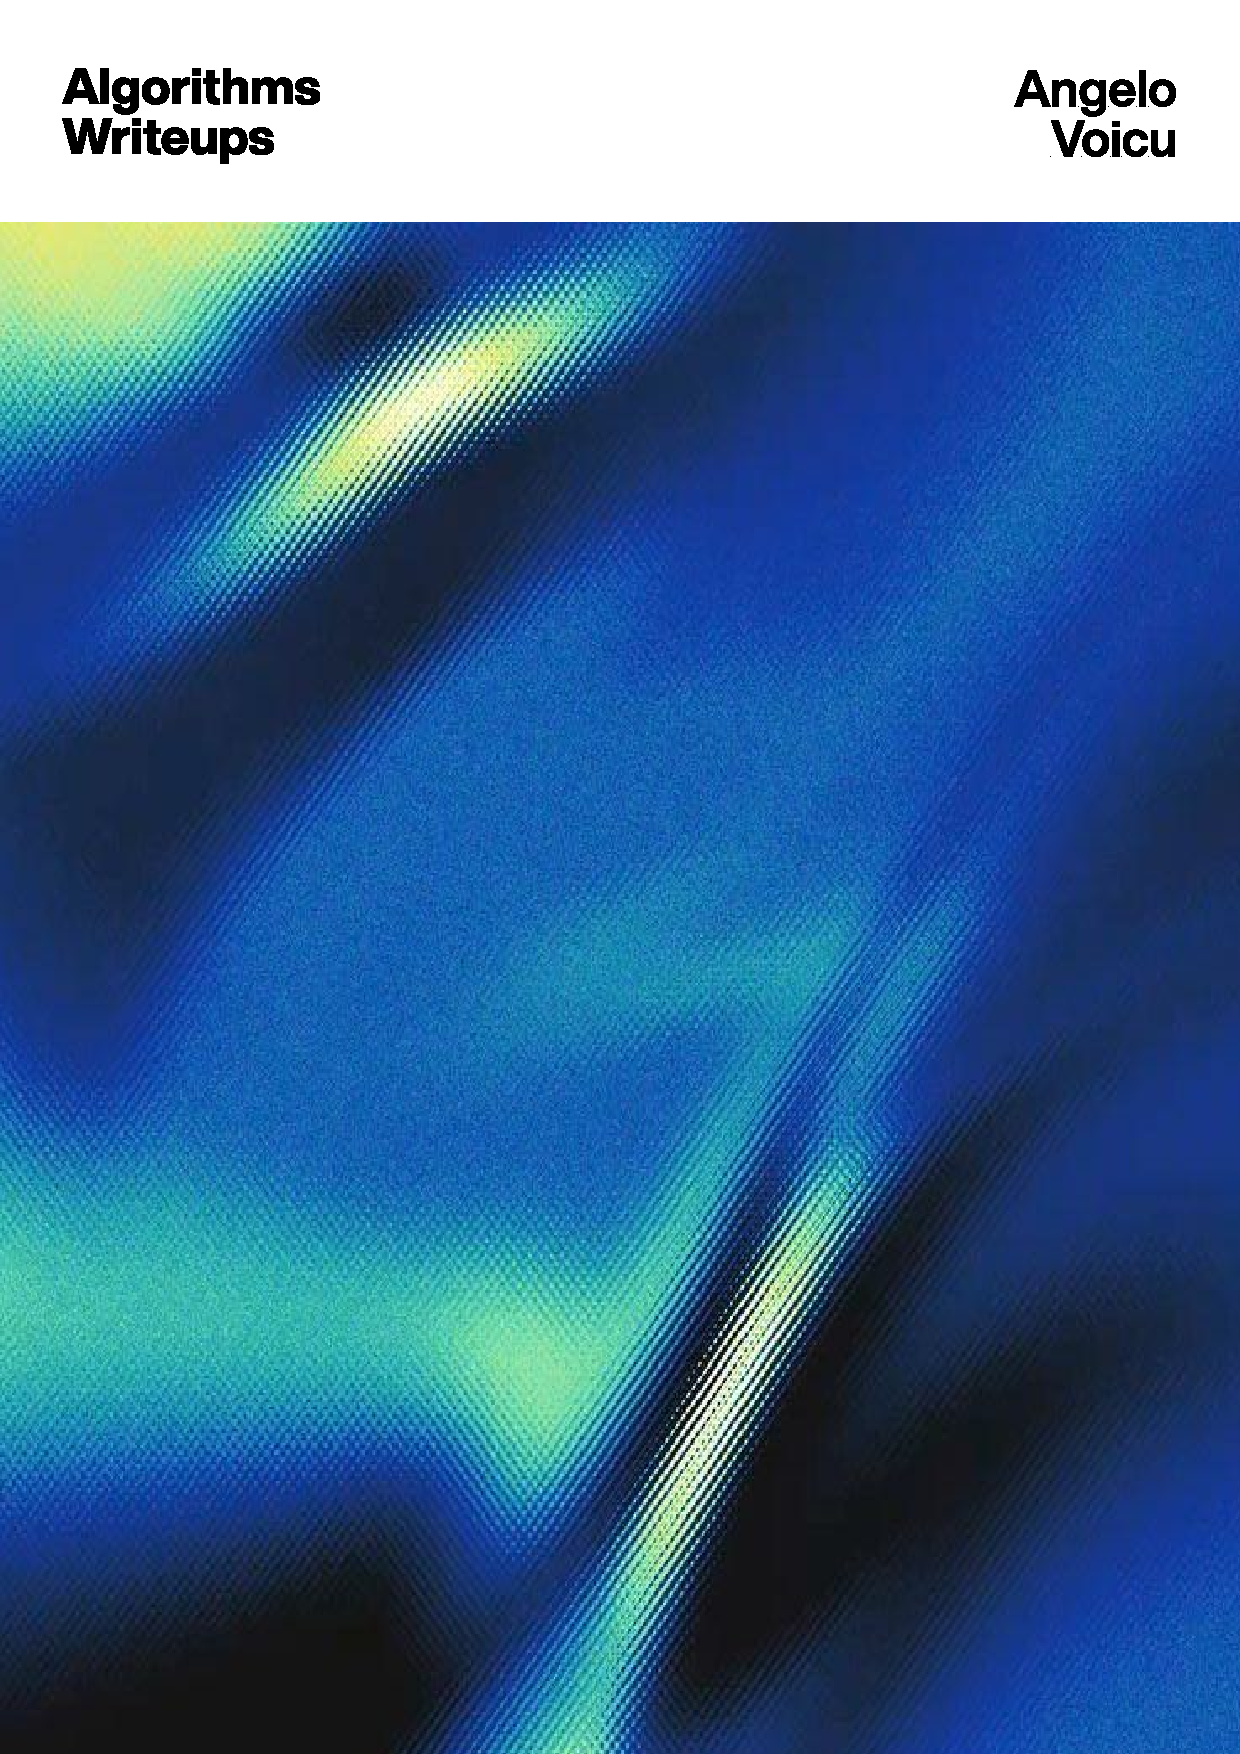
\includegraphics[width=\paperwidth]{Pictures/cover.pdf}}; % Background image
\end{tikzpicture}};
\end{tikzpicture}
\vfill
\endgroup

%----------------------------------------------------------------------------------------
%	COPYRIGHT PAGE
%----------------------------------------------------------------------------------------

\newpage
~\vfill
\thispagestyle{empty}

\noindent Copyright \copyright\ 2013 John Smith\\ % Copyright notice

\noindent \textsc{Published by Publisher}\\ % Publisher

\noindent \textsc{book-website.com}\\ % URL

\noindent Licensed under the Creative Commons Attribution-NonCommercial 3.0 Unported License (the ``License''). You may not use this file except in compliance with the License. You may obtain a copy of the License at \url{http://creativecommons.org/licenses/by-nc/3.0}. Unless required by applicable law or agreed to in writing, software distributed under the License is distributed on an \textsc{``as is'' basis, without warranties or conditions of any kind}, either express or implied. See the License for the specific language governing permissions and limitations under the License.\\ % License information

\noindent \textit{First printing, March 2013} % Printing/edition date

%----------------------------------------------------------------------------------------
%	TABLE OF CONTENTS
%----------------------------------------------------------------------------------------

%\usechapterimagefalse % If you don't want to include a chapter image, use this to toggle images off - it can be enabled later with \usechapterimagetrue

\chapterimage{chapter_head_1.pdf} % Table of contents heading image

\pagestyle{empty} % No headers

\tableofcontents % Print the table of contents itself

\cleardoublepage % Forces the first chapter to start on an odd page so it's on the right

\pagestyle{fancy} % Print headers again

%----------------------------------------------------------------------------------------
%	PART
%----------------------------------------------------------------------------------------

\part{Part One}


%----------------------------------------------------------------------------------------
%	CHAPTER 1
%----------------------------------------------------------------------------------------

\chapterimage{chapter_head_2.pdf} % Chapter heading image

\chapter{Greedy algorithms}

\section{Warmup problems}
\subsection{C. Racing}
\url{https://codeforces.com/contest/2110/problem/C} \\

We have a drone that starts at height $h_0 = 0$ and it traverses obstacles for $i = 1..n$ so its height has to change to stay between $l_i, r_i$, so we have the constraint
\begin{center}
    $l_i \leq h_i \leq r_i$.
\end{center}

We are also given an array $d_i = h_i - h_{i-1} = 0\ \lor\ 1$ that represent the deltas in heights of the drone; it is eiher 0 or 1 so this means that the height remains the same or increases by 1: it's a non-decreasing function. This array $d_i$ is not complete but has holes in it represented by -1s. The goal is to fill the holes with 0 or 1 s.t. the drone has a height $l_i \leq h_i \leq r_i\ \forall i=1..n$.

\subsubsection{Approach 1}
One could try to increment $h_i$ at each step $i$ if possible by keeping $h_i \leq \min_{i \in [i..n]}(r_i)$ but this turns out to be incorrect because if we have input $d= [-1, 1]$ and an array of constraints $(l_i,r_i)$ like $[(0,1), (0,1)]$, then we would increase by 1 at the first step because $\min_{i \in [1..2]}(r_i) = 1$, making $d' = [1, 1]$ $\implies$ $h_2 =d'_1 + d'_2 = 2 > r_2 =1$ and this violates the constraint.

\subsubsection{Approach 2}
Let's consider another approach: suppose we are in the middle of the race at step $j$. At this step we have height $h_j$ and how did we get to this height? By summing the $d_i \neq -1$ we were given and by summing the undetermined $d_i$ (those $= -1$). So at each step:
\begin{itemize}
    \item While the current height $< l_i$ we transform the preceding $-1$s and transform them into $1$s.
    \item While the (current height + no. of $-1$s seen until now) $> r_i$ we transform the preceding $-1$s into $0$s. 
\end{itemize}


So in short, what we do is $\forall i$ we consider the current $h_i$. If we are too low, we substitute $-1$s with $1$. If (height + \# of $-1$s) $> r_i$ we are too high, this means that some of the $-1$s need to be 0s because if they were all 1s we would have $h_i = \sum_{j=1}^{i}{d_j} > r_i$ which violates the constraint. So it has to be that those -1s have to be transformed into 0s. If we can't do this because we haven't got enough $-1$s we output that it's impossible.

\begin{minted}{c++}
#include <bits/stdc++.h>
using namespace std;
using ll=long long;
#define debug(x) cout << #x << " = " << x << '\n';
#define vdebug(a) cout << #a << " = "; for(auto x: a) cout << x << " "; cout << '\n';
 
void test_case() {
  ll n; cin >> n;
  vector<ll> d(n);
  for (ll &x : d) cin >> x;
  vector<ll> l(n), r(n);
 
  for (ll i = 0; i < n; i++)
    cin >> l[i] >> r[i];
  
  vector<ll> indices;
  ll height = 0; // the cumulative height
  for (ll i = 0; i < n; i++) {
    if (d[i] == -1)  {
      indices.push_back(i);
    } else {
      height += d[i];
    }
 
    while (height < l[i]) {
      if (indices.empty()) {
        cout << "-1\n";
        return;
      }
 
      d[indices.back()] = 1;
      height++;
      indices.pop_back();
    }
 
    while (height + indices.size() > r[i]) {
      if (indices.empty()) {
        cout << "-1\n";
        return;
      }
 
      d[indices.back()] = 0;
      indices.pop_back();
    }
  }
 
  for (ll x : d) {
    cout << max(0LL, x) << " ";
  }
  cout << endl;
}
 
int32_t main() { /* Omitted for brevity */ }
\end{minted}

\subsection{C. You Soared Afar With Grace}
\url{https://codeforces.com/problemset/problem/2084/C} \\

We are given two permutations $a$ and $b$ and we are asked to make them so that a and b are reverses of each other. We can do the operation
\begin{center}
    swap($a_i$, $a_j$) \\
    swap($b_i$, $b_j$)
\end{center}
where $1 \leq i,j \leq n$ and $i \neq j$ at most $n$ times. The problem asks if it is possbile to make such a and b and if it's impossible to output $-1$.

What we do is observing that each pair ($a_i$, $b_i$) has to have a corresponding ($b_i$, $a_i$) for this to work. The thing is 

\begin{minted}{C++}
#include <bits/stdc++.h>
using namespace std;
using ll=long long;
#define debug(x) cout << #x << " = " << x << '\n';
#define vdebug(a) cout << #a << " = "; for(auto x: a) cout << x << " "; cout << '\n';
#define x first
#define y second

void test_case() {
  ll n; cin >> n;
  vector<pair<ll, ll>> a(n);

  for (ll i = 0; i < n; i++) cin >> a[i].x;
  for (ll i = 0; i < n; i++) cin >> a[i].y;

  map<pair<ll, ll>, ll> pos;
  for (ll i = 0; i < n; i++) 
    pos[{a[i].x, a[i].y}] = i;

  vector<pair<ll, ll>> ans;
  for (ll i = 0; i < n; i++) {
    ll new_pos_for_brother = n - 1 - i; 
    ll pos_of_brother = pos[{a[i].y, a[i].x}];

    if (a[i].x == a[i].y) {
      pos_of_brother = i;
      new_pos_for_brother = n / 2;
    }
    
    if (pos_of_brother != new_pos_for_brother) {
      ans.push_back({pos_of_brother, new_pos_for_brother});

      swap(a[pos_of_brother], a[new_pos_for_brother]);
      swap(pos[a[pos_of_brother]], pos[a[new_pos_for_brother]]);
    }
  }
  
  bool flag = 1;
  for (ll i = 0; i < n; i++) {
    flag &= (a[i].x == a[n-1-i].y);
  }

  if (!flag) {
    cout << "-1\n";
    return;
  }

  cout << ans.size() << endl;
  for (auto el : ans) 
    cout << el.x + 1 << " " << el.y + 1 << endl;
}

int32_t main() { /* Omitted for brevity */ }
\end{minted}

\subsection{2034C - Trapped in the Witch's Labyrinth}
\url{https://codeforces.com/problemset/problem/2034/C} \\

Here what we do is build a graph and connect those nodes that have a path to the exit of the maze. We represent the exit as a separate node: the exit node. Then, we color red the nodes that are linked to the exit node, and white the ones that don't have a path to the exit. The answer will be the no. of the white nodes = $n \times m -$ (no. of red nodes).

\begin{minted}{c++}
#include <bits/stdc++.h>
using namespace std;
using ll=long long;
#define debug(x) cout << #x << " = " << x << '\n';
#define vdebug(a) cout << #a << " = "; for(auto x: a) cout << x << " "; cout << '\n';

class Graph {
public:
  map<ll, vector<ll>> adj_list;
  map<ll, bool> visited;
  map<ll, bool> node_label; // 0 = white, 1 = red
  
  void insert_node(ll x) { 
    if (adj_list.count(x) == 0) {
      adj_list[x] = {};
    }
  }

  void add_neighbour(ll x, ll neigh) {
    adj_list[x].push_back(neigh);
  }

  void print() {
    for (auto p : adj_list) {
      cout << "" << p.first << ": [ "; 
      for (ll node : p.second) cout << node << " ";
      cout << "]\n";
    }
  }

  bool dfs(ll node) {
    if (node == 0) return true;
    visited[node] = true;

    for (ll n : adj_list[node]) {
      bool neigh_is_red = 0;
      if (visited.count(n) == 0) { // v.visited == false
        neigh_is_red = dfs(n);
      } 
      
      if (neigh_is_red || (visited[n] && node_label[n] == 1)) {
        node_label[node] = 1;
        return true;
      } 
    }

    return false;
  }
}; 

void test_case() {
  ll n, m; cin >> n >> m;
  Graph g;
  g.insert_node(0);

  vector<pair<ll, ll>> int_mark_positions;

  // Let's create a graph and connect those nodes that are linked to the exit node.
  // Then, let's color red the nodes that are linked to the exit, and white the others.
  // The answer will be the no. of the white nodes = n * m - (no. of red nodes)
  for (ll y = 0; y < n; y++) {
    for (ll x = 0; x < m; x++) {
      char c; cin >> c;
      ll nx = x, ny = y; // coordinates of the neighbor pointed by the direction

      if (c == 'U') ny--;
      else if (c == 'L') nx--;
      else if (c == 'R') nx++;
      else if (c == 'D') ny++;

      ll node_num = y * m + x + 1;
      if (nx < 0 || ny < 0 || nx >= m || ny >= n) {
        // this node is linked to the exit node.
        g.add_neighbour(node_num, 0);
      } else if (c == 'U' || c == 'L' || c == 'R' || c == 'D') {
        g.add_neighbour(node_num, ny * m + nx + 1);
      } else {
        int_mark_positions.push_back({x, y});
      }
    }
  }

  for (auto [node, _] : g.adj_list) {
    g.dfs(node);
  }

  ll red_nodes = 0;
  for (auto [key, v] : g.node_label) {
    if (v) red_nodes++;
  }

  const ll mx = n * m;
  for (auto [x, y] : int_mark_positions) {
    vector<pair<ll, ll>> pos = {{x, y-1}, {x, y+1}, {x-1, y}, {x+1, y}};
    vector<pair<ll, ll>> to_process;

    copy_if(pos.begin(), pos.end(), back_inserter(to_process), [n, m](const auto &point) {
      auto [x, y] = point;
      return x >= 0 && x < m && y >= 0 && y < n;
    });

    bool f = 1;
    for (auto [x, y] : to_process) {
      ll neigh_pos = y * m + x + 1;
      f &= g.node_label[neigh_pos];
    }

    if (f) red_nodes++;
  }

  cout << n * m - red_nodes << endl;
}

int32_t main() { /* Omitted for brevity */ }
\end{minted}


\subsection{2014D - Robert Hood and Mrs Hood}
\url{https://codeforces.com/problemset/problem/2014/D} \\ 
La soluzione è quella di creare degli array di frequenze in base alle $l_i$, $r_i$ lette. Quindi avremo due vettori $o[]$, $c[]$ che contano il numero di aperture, o chiusure rispettivamente, al giorno $i$. Quindi, facciamo le prefix sum degli array e ciò ci apre la possibilità di ottenere quanti jobs ci sono tra $i$ e $i-d$ facendo 
\begin{equation}
    \quad \quad \text{\# di jobs nell'intervallo} [i - d..i] = o[i] - c[i-d].
\end{equation}

\begin{minted}{c++}
#include <bits/stdc++.h>
using namespace std;
using ll=long long;
#define debug(x) cout << #x << " = " << x << '\n';
#define vdebug(a) cout << #a << " = "; for(auto x: a) cout << x << " "; cout << '\n';
typedef vector<ll> vi;
typedef pair<ll, ll> pi;

void test_case() {
  ll n, d, k; cin >> n >> d >> k;
  vi o(n+1), c(n+1);
  for (ll i = 0; i < k; i++) {
    ll a, b; cin >> a >> b;
    o[a]++;
    c[b]++;
  }

  for (ll i = 0; i < n; i++) o[i+1] += o[i];
  for (ll i = 0; i < n; i++) c[i+1] += c[i];

  ll mx = 0, mn = LLONG_MAX;
  ll brother, mother;
  for (ll i = d; i <= n; i++) {
    ll curr = o[i] - c[i-d];

    if (curr > mx) mx = curr, brother = i-d+1;
    if (curr < mn) mn = curr, mother = i-d+1;
  }

  cout << brother << " " << mother << "\n";
}

int32_t main() { /* Omitted for brevity */ }
\end{minted}

\subsection{E - Kirei Attacks the Estate}
\url{https://codeforces.com/problemset/problem/2114/E} \\
We define two functions $f$, $g$ like so, where $f(v)$ is the maximum alternating sum for node $v$.
\begin{equation}
\begin{matrix}
    f(v) = \max(a_v, a_v - g(p_v)) \\ 
    g(v) = \min(a_v, a_v - f(p_v))
\end{matrix}
\end{equation}

In the end $f$ and $g$ are represent the same expression just negated and include the $\min$, $\max$ operators so that we can maximize the overall sum. 

By expanding 3 times we get,
\begin{align*}
    f(v) &= \max\Big(a_v,\, a_v - \big(\min\big(a_{p_v},\, a_{p_v} - \max(a_{p_{p_v}},\, a_{p_{p_v}} - g(p_{p_v}))\big)\big)\Big)\\
    &= \max\Big(a_v,\, a_v + \min\big(-a_{p_v},\, -a_{p_v} + \max(a_{p_{p_v}},\, a_{p_{p_v}} - g(p_{p_{p_v}}))\big)\Big)
\end{align*}

so we end up with a sequence like,
\begin{align*}
    a_v - a_{p_v} + a_{p_{p_v}} - \dots 
\end{align*}
where we want to maximize the positive terms and minimize the negative ones.

\begin{obs}
    If you pay attention closely to the formula you can see that 
    \begin{equation}
        -g(v) = \min(-a_v, -a_v + f(p_v))
    \end{equation}
    is trying to choose between something negative and something negative plus something $\geq 0 $. This is redundant, so we can just re-define $g$ as
    \begin{equation}
    \begin{matrix}
        -g(v) = -a_v + f(p_v) \\
        g(v) = a_v - f(p_v) 
    \end{matrix}
    \end{equation}

    and thus we could change the corresponding expr in the code below.

    So expanding and substituting we get the expression,
    \begin{equation}
        \max\Big(a_v, a_v - a_{p_v} + \max\big(a_{p_{p_v}}, a_{p_{p_v}} - g(p_{p_{p_v}}) \big) \Big).
    \end{equation}
\end{obs}

\begin{obs}
    Takeaway: when you have an alternating sum such as
    \begin{equation}
        a -b+c-d+\dots
    \end{equation}
    you maximise the $\geq 0$ terms and minimize the $\leq 0$ terms.
    This was done by creating two arrays, f and g and storing two expressions, first the positive one and then the negative one.
\end{obs}

\begin{minted}{c++}
#include <bits/stdc++.h>
using namespace std;
using ll=long long;
#define debug(x) cout << #x << " = " << x << '\n';
#define vdebug(a) cout << #a << " = "; for(auto x: a) cout << x << " "; cout << '\n';
typedef vector<ll> vi;
typedef pair<ll, ll> pi;

class Tree {
public:
  map<ll, vi> adj_list;
  vi visited;
  vi f, g, a;

  Tree(ll n, vi& a) {
    visited.resize(n+1, 0);
    f.resize(n+1, 0);
    g.resize(n+1, 0);
    this->a = a;

    f[1] = g[1] = a[1];
  }

  void add_node(ll u, ll v) {
    adj_list[u].push_back(v);
    adj_list[v].push_back(u);
  }

  void print() {
    for (auto k : adj_list) {
      cout << k.first << ": ";
      for (ll n : k.second) {
        cout << n << " ";
      }

      cout << endl;
    }
  }

  void dfs(ll node, ll parent) {
    visited[node] = 1;

    if (node != 1) {
      f[node] = max(a[node], a[node] - g[parent]);
      g[node] = min(a[node], a[node] - f[parent]);
      // or: g[node] = a[node] - f[parent];
    }

    for (ll n : adj_list[node]) {
      if (!visited[n]) 
        dfs(n, node);
    }
  }
};

void test_case() {
  ll n; cin >> n;
  vi a(n+1); for (ll i = 1; i <= n; i++) cin >> a[i];

  Tree t(n, a);

  for (ll i = 0; i < n - 1; i++) {
    ll a, b;
    cin >> a >> b;

    t.add_node(a,b);
  }

  t.dfs(1, 1);
  for (ll i = 1; i <= n; i++) cout << t.f[i] << " ";
  cout << "\n";
}

int32_t main() {
  ios_base::sync_with_stdio(0); cin.tie(0);

  int t;
  cin >> t;
  while (t--) {
    test_case();    
  }
}
\end{minted}

\subsection{Swapping Brackets}
\url{https://training.olinfo.it/task/ois_bracketswap}

We first begin taking strings and playing around swapping parentheses. We keep a count and decrease it when we encounter a closing parenthesis, and increase it when we find an open one. We observe that,

\begin{obs}
    The counter becomes negative $\iff$ $s$ is invalid. \\
    And obviously, \\
    s is valid $\iff$ The counter is always non-negative.
\end{obs}

From here we also observe that if we have a certain count $x$, and we have a closing parenthesis after the count will become $x-1$, if we have an open instead the count will be $x + 1$. If we swap the two parentheses at indexes $i, j$ it means that all the counts between $i$ and $j$ will be increased by $(x + 1) - (x - 1)  = 2$. Draw a diagram where you substitute parenthesis with arrows (up and down) and it will be clear why.
\\
Let's call $count_k$ the count we have up until index $k$. The number of steps to solve the problem is just,
\begin{equation}
    \Bigl\lfloor \frac{ (- \min_{k}\{count_k\}) + 1}{2} \Bigr\rfloor
\end{equation}

The implementation of this formula is in the \texttt{steps} function.

\begin{minted}{c++}
#include <bits/stdc++.h>
using namespace std;
using ll=long long;
#define debug(x) cout << #x << " = " << x << '\n';
#define vdebug(a) cout << #a << " = "; for(auto x: a) cout << x << " "; cout << '\n';
typedef vector<ll> vi;
typedef pair<ll, ll> pi;

ll steps(string s, ll n) {
  ll ret = LLONG_MAX;
  ll counter = 0;

  for (ll i = 0; i < n; i++){
    if (s[i] == '(') counter++;
    else counter--;

    ret = min(ret, counter);
  }

  return ((-(ret) + 1) / 2);
}

void test_case() {
  ll n; cin >> n;
  string s; cin >> s;

  stack<ll> opening; // indexes

  for (ll i = 0; i < n; i++) {
    if (s[i] == '(') opening.push(i);
  }

  ll t = steps(s, n);
  cout << t << "\n";

  for (ll i = 0; i < n / 2 && t > 0; i++) {
    if (s[i] == ')') {
      ll opidx = opening.top();
      opening.pop();

      swap(s[opidx], s[i]);
      cout << i << " " << opidx << "\n";
      t--;
    }
  }
}

int32_t main() { test_case(); }
\end{minted}

\subsection{D. Temple Architecture}
\url{https://codeforces.com/gym/105677/problem/D} \\

\begin{problem}
    For each element in a list $H$, find the nearest greater element.
\end{problem}

The problem can be solved using a greedy algorithm that first computes the nearest greater element considering only the elements to the left of a given $H_i$ and then considering only the elements to the right. 
Let's consider the first part. We use a stack and we range $i = 0..n-1$ we remove an element from the stack when $H_j \leq H_i$ because if after $H_i$ we have $H_{i+1} < H_i$ then the nearest greater element is $H_i$, otherwise if $H_{i+1} > H_i$ then for sure those $H_j \leq H_i$ were useless in determining the nearest greater element for $H_{i+1}$. A similar thing is done for the right side. Then we compute the answer as shown below.

\begin{minted}{c++}
#include <bits/stdc++.h>
using namespace std;
using ll=long long;
#define debug(x) cout << #x << " = " << x << '\n';
#define vdebug(a) cout << #a << " = "; for(auto x: a) cout << x << " "; cout << '\n';
typedef vector<ll> vi;
typedef pair<ll, ll> pi;

void test_case() {
  ll n; cin >> n;
  vi a(n);
  vi left(n, LLONG_MAX), right(n, LLONG_MAX);
  for (ll &x : a) cin >> x;

  // Find left boundaries (previous greater element)
  stack<ll> s;
  s.push(0);

  for (ll i = 1; i < n; i++) {
    while (s.size() > 0 && a[s.top()] <= a[i])
      s.pop();

    if (s.size() > 0)
      left[i] = s.top();
    s.push(i);
  }

  // Clear stack for right boundaries
  while (!s.empty()) s.pop();
  
  // Find right boundaries (next greater element)
  s.push(n - 1);
  for (ll i = n - 2; i >= 0; i--) {
    while (s.size() > 0 && a[s.top()] <= a[i])
      s.pop();

    if (s.size() > 0)
      right[i] = s.top();
    s.push(i);
  }

  ll ans = 0;
  ll p = max_element(a.begin(), a.end()) - a.begin();
  for (ll i = 0; i < n; i++) {
    if (i != p) {
      ll x = min(left[i] != LLONG_MAX ? (i - left[i]) : LLONG_MAX, 
                 right[i] != LLONG_MAX ? (right[i] - i) : LLONG_MAX);

      ans += x;
    }
  }

  vdebug(right)
  
  cout << ans << "\n";
}

int32_t main() {
  ios_base::sync_with_stdio(0); cin.tie(0);
  test_case();
}   
\end{minted}


\section{Binary search}

\subsection{Christmas lights}
\url{https://training.olinfo.it/task/ois_lights}
\\

The problem gives us a strip of Christmas lights of length $n$, represented as an integer array. We're asked to find the minimum length of a contiguous subarray that contains all numbers in the range $[0, c-1]$, where $c$ is given.

To solve this, we can perform a binary search on the answer—i.e., on the length of the subarray. This approach is valid because of the following observation:

If there exists a valid subarray of length $x$ that contains all required numbers, then any subarray of length $x+1$ (that contains the same elements and possibly more) can also be valid. That is, the property of being valid is monotonic with respect to length:

$$ x \text{ valid}  \implies x+1 \text{ valid} $$

This monotonicity allows us to apply binary search over possible subarray lengths. For each candidate length, we can check using a sliding window whether there exists a subarray of that length that includes all numbers from $0$ to $c-1$.

In order to check there exists a valid subarray of length $sz$, we use the following observation
\begin{obs}
    The variant when we slide the window is that we decrease the frequency of the left end element just removed and increase the frequency of the new element added. To determine whether the current window is valid, we keep track of how many of the required values in $[0, c - 1]$ are still missing from the window (this can be done in $O(1)$). If the number of missing values is equal to 0 then the window is valid and we return true.
\end{obs}

The complexity is
$$ O(\log n) \cdot O(n)$$.
\begin{minted}{c++}
void test_case() {
  ll n, c; cin >> n >> c;
  vi a(n), freq(c);
  for (ll &x : a) cin >> x;

  // Given the size of the window, slide it and output if its valid.
  auto valid = [&](ll sz) {
    vi freq(c);
    bool valid = 1;
    ll missing = 0; // # of spots in freq where freq[i] == 0.

    for (ll i = 0; i < sz; i++) freq[a[i]]++;
 
    for (ll f : freq) {
      valid &= (f > 0);
      if (f == 0) missing++;
    }
    
    if (valid) return true;

    for (ll i = 1; i < n - sz && !valid; i++) {
      
      // Remove one element from the window
      freq[a[i-1]]--;
      if (freq[a[i-1]] == 0) missing++;
      
      // Add one element to the window
      if (freq[a[i+sz-1]] == 0) missing--;
      freq[a[i+sz-1]]++;
      
      // If we have all the numbers in [0..C-1] in the window 
      // then we return true
      if (missing == 0) valid = 1;
    }

    return valid;
  };

  ll l = c, r = n;
  ll mn = LLONG_MAX; // Minimal subarray length
  while (l <= r) {
    ll mid = (l + r) / 2;

    if (valid(mid)) {
      mn = min(mn, mid);
      r = mid - 1;
    } else {
      l = mid + 1;
    }
  }

  cout << mn << endl;
}
\end{minted}

\subsection{Save the barrels}
\url{https://training.olinfo.it/task/ois_butoaie}\\ 

There's no particular contraints on $P$ and $Q$ i.e. it can be $P\ \substack{< \\ = \\ >}\  Q$; so what we do is assuming $P > Q$, if this is not the case we swap $P$ and $Q$.

What we know is we have an array $V[]$ on which we can use, every day, $K$ diffusers of power $P$ and $N - K$ of power $Q$. After a certain number of days we wanna have all $V_i = 0$. So this means subtracting a certain number of $P$s and $Q$s from $V_i$.
$$V_i - P \cdot d_i - Q \cdot b_i = 0$$

Here $d_i$, $b_i$ are the number of diffusers of power $P$ and $Q$ respectively we use on day $i$. 

\begin{idea}
    Let $x$ = no. of days to use the available diffusers so that we make all $V_i = 0$. Then let's binary search on $x$.
\end{idea}

Note that it has to be that $b_i + d_i = x\ \forall i$.

From the two equations we just shown we get
$$ V_i - P \cdot d_i - Q \cdot b_i = 0 $$
$$ V_i - P \cdot d_i - Q \cdot (x - d_i) = 0$$
$$ d_i = \ceil[\Bigg]{\frac{V_i - Qx}{P - Q}} $$

We take the ceiling of the result just because $d_i$ could be decimal and we can't use, say, half a diffuser.

Then we make the following observations,

\begin{gather*}
\underbrace{\sum_i d_i}_{\text{\# of strong diffusers we want to use}} 
\leq 
\underbrace{K \cdot x}_{\text{\# of strong diffusers available}}
\\
\underbrace{d_i}_{\text{\# of diffusers used on day } i} \leq x
\end{gather*}

and we notice that if $V_i \leq Qx$ (i.e. we may use only weak diffusers to make $V_i = 0$), so we don't need to calculate the value of $d_i$ (= no. of strong diffusers needed to make $V_i = 0$).

\begin{minted}{c++}
#include <bits/stdc++.h>
using namespace std;
using ll=long long;
#define debug(x) cout << #x << " = " << x << '\n';
#define vdebug(a) cout << #a << " = "; for(auto x: a) cout << x << " "; cout << '\n';
typedef vector<ll> vi;
typedef pair<ll, ll> pi;

void test_case() {
  ll n, k, p, q; cin >> n >> k >> p >> q;
  vi a(n);
  for (ll &x : a) cin >> x;

  ll nstrong = k, nweak = n - k;
  
  if (p < q) {
    swap(p, q);
    swap(nstrong, nweak);
  }

  // Is it possible to complete the task in a certain amount of days?
  auto valid = [&](ll days) -> bool {
    ll sumd = 0;

    for (ll &v : a) {
      if (v <= q * days) continue;
      
      ll d = ceil((long double)(v - q * days) / (p - q));

      if (d > days) return false;
      sumd += d;
    }

    return sumd <= nstrong * days;
  };

  ll l = 0, r = 1e12; 
  
  while (l <= r) {
    ll mid = (l + r) / 2;

    if (valid(mid)) {
      r = mid - 1; 
    } else {
      l = mid + 1;
    }
  }

  cout << r + 1 << endl;
}

int32_t main() {
  ios_base::sync_with_stdio(0); cin.tie(0);
  test_case();
}
\end{minted}

\subsection{D. Beautiful Permutation - Searching for only one endpoint}
\url{https://codeforces.com/contest/2162/problem/D}

Here what we can do is a binary search where we calculate $p - a$ in the range $[l, r]$ thus doing,
\begin{align*}
    &\text{query}(1, 1, m) \\ 
    &\text{query}(1, m+1, n) \\ 
    &\text{query}(2, 1, m) \\
    &\text{query}(2, m+1, n) \\ 
\end{align*}

but this is too slow taking $4 \cdot \lceil \log_2(n) \rceil > 40$ operations.

Another approach is looking only for $l$ by comparing $\text{query}(1, 1, m)$ and $\text{query}(2, 1, m)$. And then calculating r as $ r = l + \text{\# of 1s}$.

\begin{minted}{c++}
void test_case() {
  ll n; cin >> n;
  
  auto query = [&](ll type, ll l, ll r) -> ll {
    cout << type << " " << l << " " << r << endl;
    ll x; cin >> x;
    return x;
  }; 
  
  ll sum = query(2, 1, n) - ((n * (n + 1)) / 2);

  ll l = 1, r = n;

  while (l < r) {
    ll m = (l + r) / 2;
    ll a = query(1, 1, m), b = query(2, 1, m);

    if (a < b) r = m;
    else l = m + 1;
  }
  
  cout << "! " << l << " " << l + sum - 1 << endl;
}
\end{minted}

\section{Minimax problems with binary search}
Minimax problems are those where we have to minimize a maximum value or maximize a minimum value. Let's consider a classical problem. \\ 

\begin{problem}
    Given an array $a$ of positive integers and an integer $k$, split the array into $k$ contiguous subarrays. Your goal is to minimize the largest sum among these subarrays.
\end{problem}

So here we have to \textbf{minimize} the \textbf{maximum} sum of $b^j$ subarray of $a$.

\begin{minted}{c++}
void test_case() {
  ll n, k; cin >> n >> k;
  vi nums(n);
  for (ll &x : nums) cin >> x;
  
  auto check = [&](ll x) -> bool {
    ll i = 0;
    ll currk = 0;

    while (i < n) {
      ll currsum = 0;
      while (currsum < x && i < n) {
        currsum += nums[i];
        if (currsum <= x) i++;
      }

      while (nums[i] == 0 && i < n) i++;
      
      currk++;
    }

    return currk <= k;
  };

  ll l = *max_element(nums.begin(), nums.end()), 
     r = accumulate(nums.begin(), nums.end(), 0LL);
  
  while (l <= r) {
    ll mid = (l + r) / 2;

    if (check(mid)) {
      r = mid - 1;
    } else {
      l = mid + 1;
    }
  }

  cout << r + 1 << endl;
}
\end{minted}



\subsection{E. Min Max MEX}
\begin{sloppypar}
\url{https://codeforces.com/problemset/problem/2093/E}
\end{sloppypar}

\begin{minted}{c++} 
bool seen[200005];

void test_case() {
  ll n, k; cin >> n >> k;
  vi a(n);
  for (ll &x : a) cin >> x;

  memset(seen, 0, 200005);

  auto check = [&](ll x) -> bool {
    ll subarrays = 0;
    ll i = 0;
    
    while (i < n) {
      ll count_seen = 0;

      while (i < n) {
        if (a[i] < x && seen[a[i]] == 0) {
          seen[a[i]] = 1;
          count_seen++;
        }

        i++;
        if (count_seen == x) {
          subarrays++;
          break;
        }
      }

      memset(seen, 0, min(x + 1, (ll) 2e5) * sizeof(bool));
    }
    
    memset(seen, 0, min(x + 1, (ll) 2e5) * sizeof(bool));
    return subarrays >= k;
  };

  
  ll l = 0LL, r = 2e5;
  while (l <= r) {
    ll mid = (l + r) / 2;

    if (check(mid)) {
      l = mid + 1;
    } else {
      r = mid - 1;
    }
  }

  cout << l - 1 << endl;
}
\end{minted}
\chapterimage{chapter_head_1.pdf} % Chapter heading image
\chapter{Dynamic programming}

\subsection{A. Gellyfish and Flaming peony}
\begin{sloppypar}
\url{https://codeforces.com/problemset/problem/2115/A} 
\end{sloppypar}

It can be shown that ultimately all elements become 
$$ G = \gcd(a_1, a_2, \ldots, a_n). $$
\begin{obs}
If there is an element \( a_k = G \), then all the other elements will become \( G \).  
We just need to count the number of elements where \( a_i \neq G \ \forall i \).
\end{obs}

But if initially \( G \notin a \), then we have to calculate the number of operations to make an element in \( a \) equal to \( G \).  
We can do this using dynamic programming,
$$ f(x) = \text{\# of operations to make an element in } a \text{ equal to } x. $$

the transition equation is
$$ f(\gcd(x, a_i)) = f(x) + 1 $$

computed \( \forall x \in [\max(a) \dots 1], \quad \forall i \in \{1, 2, \ldots, n\} \)  
by updating when we find a smaller value at every iteration.

In addition, \( \gcd(a, b) \) takes \( \log(a) \) time so we need to preprocess the \texttt{gcd} function to avoid the complexity. To compute the 2 nested \texttt{for} loops will take
\[
\mathcal{O}(n \cdot \max(a) \cdot \log(\max(a)))
\]

We create a matrix for which
$$ \gcd[x][y] = \gcd[y][x] = \gcd[y][x \bmod y] $$

and this takes \( \mathcal{O}(\max(a) \cdot n) \), but we have the constraints:  
$$ 1 \leq a_i, n \leq 5000, $$
so the complexity is really  
\[
\mathcal{O}(\max(a)^2) = \mathcal{O}(n^2), \quad \text{which will be at most } (5 \cdot 10^3)^2 = 25 \cdot 10^6 \text{ operations, which is acceptable.}
\]

Therefore, we would have:
\[
\begin{array}{c|c}
\textbf{Preprocessing} & \textbf{Per Test Case} \\
\hline
\mathcal{O}(\max(a)^2) = \mathcal{O}(n^2) & \mathcal{O}(n \cdot \max(a)) = \mathcal{O}(n^2)
\end{array}
\]
\[
= \mathcal{O}(n^2) + \mathcal{O}(n^2) = \mathcal{O}(n^2)
\]

You can visualize the solution as: there is a chain of operations you do that interconnects the elements in a, and to get to g you choose one of the chains.
If you visualize it so, there are a lot of paths to take, and we eventually could arrive at the same number \( x_k \) via different paths; but in general for a specific point you are in the chain, you want the minimum cost out of all the possible paths.

And how can you take all the good possible paths? \\
By enumerating all possible \( x \)'s and all possible \( a_i \)'s.

\begin{obs}
    We know $\gcd(x, a_i) \leq x$ hence the choice of enumerating x from $\max(a)$ to $1$. Because we first fill $f(x)$ and then we can use those values to fill $f(gcd(x, a_i))$.
\end{obs}


\begin{minted}{C++}
#include <bits/stdc++.h>
using namespace std;
using ll=long long;
#define debug(x) cout << #x << " = " << x << '\n';
#define vdebug(a) cout << #a << " = "; for(auto x: a) cout << x << " "; cout << '\n';
typedef vector<ll> vi;
typedef pair<ll, ll> pi;

#define N 5005
ll g[N][N];

void test_case() {
  ll n; cin >> n;
  vi a(n), f(N, LLONG_MAX / 2LL);
  ll mx = 0, k = 0; // mx = max(a), k = gcd(a[0], ... , a[n-1])

  for (ll &x : a) {
    cin >> x;
    k = g[k][x];
  }
  
  for (ll &x : a) {
    // x /= k;
    mx = max(mx, x);
    f[x] = 0;
  } 
  
  for (ll x = mx; x >= 1; x--) {
    for (ll &y : a) {
      // remember that we want to minimize the number of operations
      if (f[g[x][y]] > f[x] + 1)
        f[g[x][y]] = f[x] + 1;
    }
  }
  
  ll ans = max(f[k] - 1, 0LL);
  for (ll &x : a) 
    if (x > k) ans++;

  cout << ans << endl;
}

int32_t main() {
  ios_base::sync_with_stdio(0); cin.tie(0);

  for (ll i=0; i<N; i++) g[i][0] = g[0][i] = g[i][i] = i;
  for (ll x=1; x<N; x++) {
    for (ll y=1; y<x; y++) {
      g[x][y] = g[y][x] = g[y][x % y];
    }
  }

  int t;
  cin >> t;
  while (t--) {
    test_case();    
  }
}
\end{minted}

\subsection{Book shop}
\begin{sloppypar}
\url{https://cses.fi/problemset/task/1158}
\end{sloppypar}

This problem is equivalent to the classical \textbf{knapsack problem}. This problem comes down to analysing 2 cases only:
\\
\begin{itemize}
    \item \textbf{Excluding the $i$-th item}, in which case the best solution is the same as the one obtained by considering only the items with indices from $1$ to $i - 1$;
    
    \item \textbf{Including the $i$-th item}, in which case the best solution is obtained by using $h_i$ units of capacity for the new item, and optimally using the remaining $j - h_i$ units of capacity for the previous items.
\end{itemize}


\begin{center}
\begin{tikzpicture}[every node/.style={font=\normalsize}]
    % Main DP formula
    \node (dp) at (0,0) {$
        \text{dp}[i][j] = \max\left(
            \begin{array}{l}
                \text{dp}[i - 1][j], \\
                \text{dp}[i - 1][j - h_i] + s_i
            \end{array}
        \right)
    $};
\end{tikzpicture}
\end{center}

where we define dp[$i$][$j$] as the maximum number of pages we can buy with $j$ dollars and including all the books from $1$ to $i$.


\subsection{Counting Towers}
\begin{sloppypar}
\url{https://cses.fi/problemset/task/2413}
\end{sloppypar}

We distinguish between type 1 towers, and type 2. Type 1 towers have the the top two cells connected, while type 2 towers have the top two cells that are part of different blocks.

\begin{figure}[!ht]
    \centering
    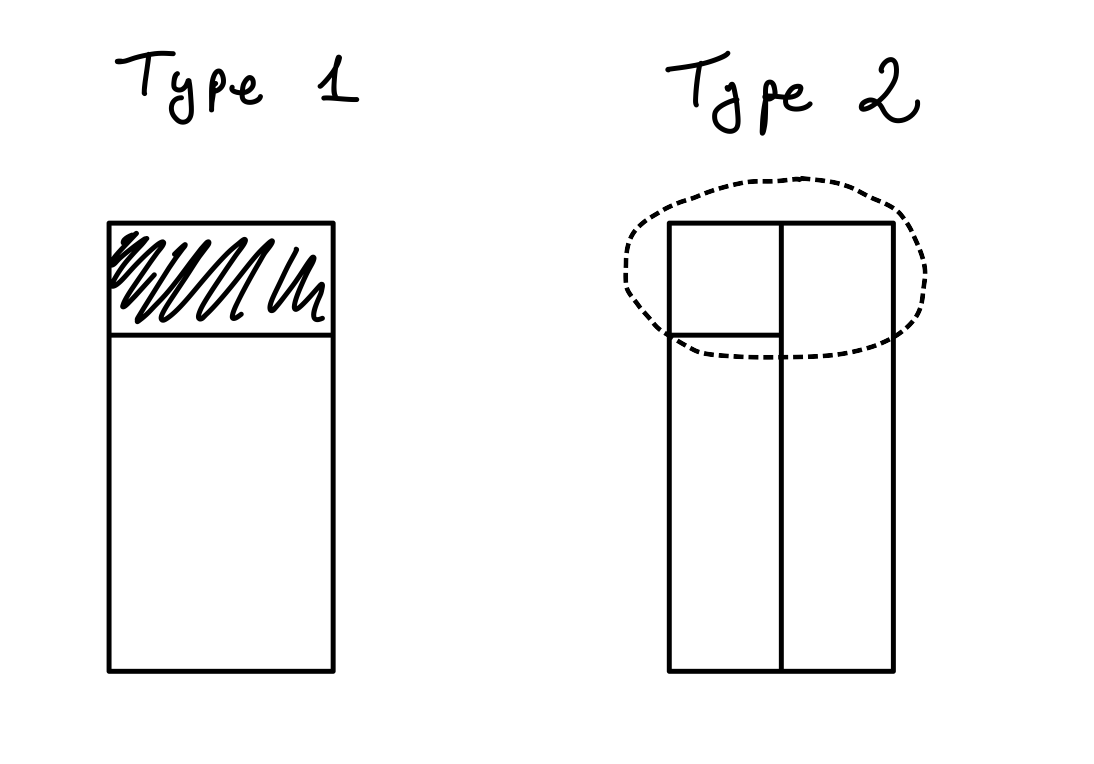
\includegraphics[width=0.5\linewidth]{Pictures/2-1.png}
    \caption{2 types of towers}
    \label{fig:21}
\end{figure}

We let $a_n$ = no. of towers of type 1 of height $n$, $b_n$ = no. of towers of type 2 of height $n$.

\begin{figure}[!ht]
    \centering
    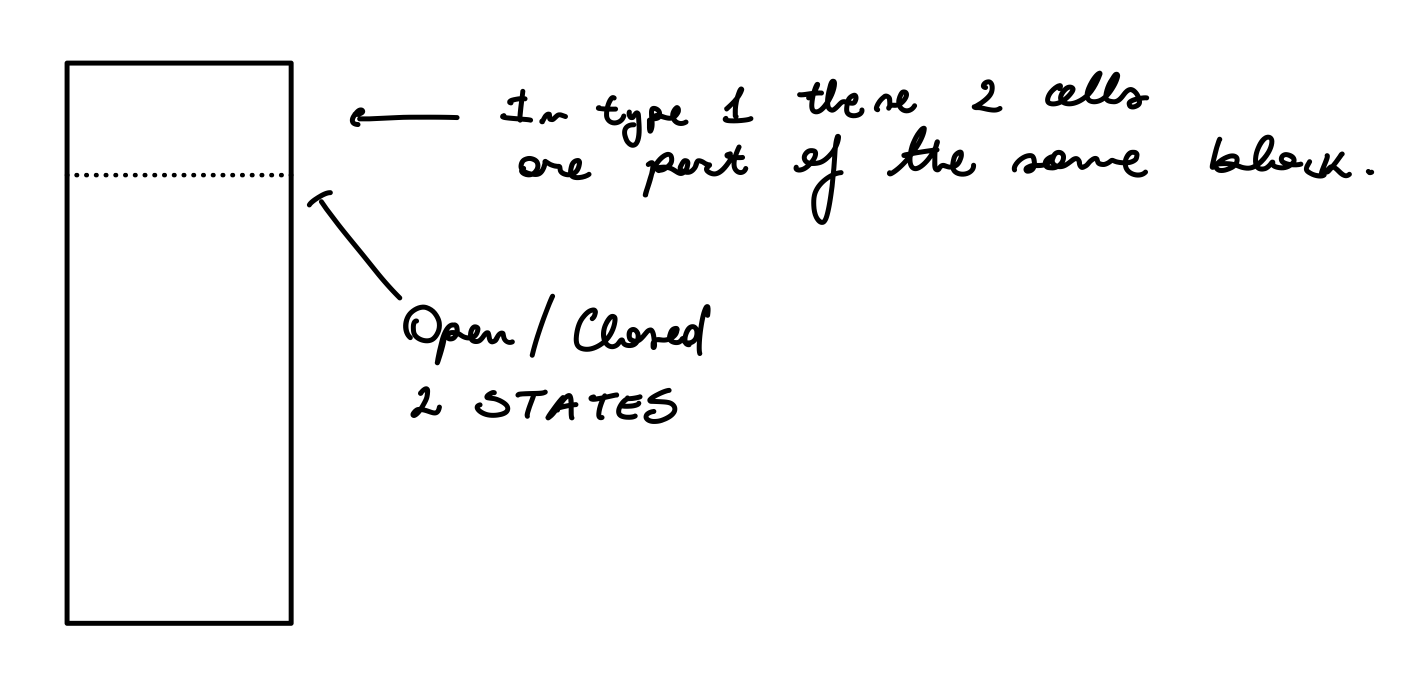
\includegraphics[width=0.75\linewidth]{Pictures/2-2.png}
    \caption{We can view the line below the $i$-th row as open or closed.}
    \label{fig:22}
\end{figure}

\subsubsection{Type 1 towers}
If we have the top 2 cells connected ($i$-th row) the dotted line (Figure \ref{fig:22}) could be empty or filled and then below it we either put a tower $(i - 1) \times 2$ of type 1. Otherwise the dotted line is filled and then we put a tower $(i - 1) \times 2$ of type 2.

\begin{equation}
    a_n = 2a_{n-1} + b_{n-1}
\end{equation}

\subsubsection{Type 2 towers}
For a type 2 tower we have a line that splits vertically the top 2 cells (see figure \ref{fig:21}) and the dotted line show in figure \ref{fig:22} can be either filled or open, leading to \textbf{4 possible states}. Below this line we could fill with type 2 towers. If we want to fill the remaining spaces with a type 1 tower we have to account for the fact that its top two cells have to be part of the same block, so the dotted line is \textit{filled}. This leads to only \textbf{1 possible state}.

\begin{equation}
    b_n = 4b_{n-1} + a_{n-1}
\end{equation}

The number of towers is $a_n + b_n$. We simply compute every value of $a_i, b_i$ leading to a complexity of $O(n)$.

\begin{minted}{c++}
#include <bits/stdc++.h>
using namespace std;
using ll=long long;
#define debug(x) cout << #x << " = " << x << '\n';
#define vdebug(a) cout << #a << " = "; for(auto x: a) cout << x << " "; cout << '\n';
typedef vector<ll> vi;
typedef pair<ll, ll> pi;

const ll mod = 1e9 + 7;

void test_case() {
  ll n; cin >> n; 
  
  ll a = 1, b = 1;
  if (n == 0) cout << "0\n";
  else if (n == 1) cout << "2\n";
  else {
    for (ll i = 2; i <= n; i++) {
      ll newa = (2*a + b) % mod;
      ll newb = (4*b + a) % mod;
  
      a = newa, b = newb;
    }
  
    cout << (a + b) % mod << endl;
  }
}
\end{minted}

\section{Constructing permutations and combinations}

\subsection{Coin combinations I \&\& II: swapping two loops can change the result!}
\begin{sloppypar}
\url{https://cses.fi/problemset/task/1635}, \url{https://cses.fi/problemset/task/1636} 
\end{sloppypar}

\subsubsection{Coin combinations I}
The first problem asks us to calculate all the distinct \textit{permutations} of a set of coins to produce a certain sum of money $x$. 
\begin{equation}
    \text{dp}[i] = \text{\# of permutations of coins that sum up to amount } i.
\end{equation}

\begin{minted}{c++}
void test_case() {
  ll n, x; cin >> n >> x;
  vector<ll> c(n);
  vector<ll> dp(x+1, 0);
  for (auto &x : c) cin >> x;

  dp[0] = 1;

  for (ll i = 1; i <= x; i++) {
    for (ll coin : c) {
      if (i - coin >= 0)
        dp[i] += (dp[i - coin] % mod);
    }
  }
  
  cout << (dp[x] % mod) << endl;
}

\end{minted}

The approach we take is iterating through the amounts $i$ ($1 \leq i \leq x$) and then trying all the possible coins to make that amount. If we want to make amount $i$, there are $\text{dp}[i - c]$ ways of doing that, where $c$ is a coin in the set that we use to complete the permutation. 
That is we are constructing all the permutations of this kind,

\begin{equation}
    (c, (\text{all the permutations that sum up to } i - c \text{ go here}))
\end{equation}


\subsubsection{Coin combinations II}

Here what's asked is to count the number of \textit{combinations} to make an amount $x$ with a given input set of coins. 

The approach we take is to select a coin $c$, and from here compute
\begin{equation}
    \text{dp}[i] = \text{\# of combinations using the given coins to reach amount } i, \forall i\ (1 \leq i \leq x). 
\end{equation}


\begin{idea}
    Here adding $3 + 1$ is the same as adding $1 + 3$, this means that we need to consider the coins in order. So we only go through the set of coins once, thus it's impossible to create two combinations with the same set of coins ordered differently. This is different from the previous problem where we considered every coin at all times.
\end{idea}

We get a time complexity of $\mathcal{O}(n \cdot x)$.

\begin{minted}{c++}
void test_case() {
  ll n, x; cin >> n >> x;
  vector<ll> c(n);
  vector<ll> dp(x+1, 0);
  for (auto &x : c) cin >> x;

  dp[0] = 1;

  for (ll coin : c) {
    for (ll i = 1; i <= x; i++) {
      if (i - coin >= 0)
        dp[i] += (dp[i - coin] % mod);
    }
  }
  
  cout << (dp[x] % mod) << endl;
}
\end{minted}

At every iteration of the outer loop we add a coin to the ones that we are using in order to construct the combinations. That is, at the first iteration we are calculating how to make all the possible amounts $1 \leq i \leq x$ only using the first coin. At the second iteration only using the first two coins, and so forth.

This means that we could have done the same job using a matrix instead of iterating on the same array multiple times by defining
\begin{equation}
    \text{dp}[j][i] = \text{\# of combinations to produce a sum of money $i$ using the first $j$ coins}.
\end{equation}

\subsection{Dice Sum}
\url{https://atcoder.jp/contests/abc248/tasks/abc248_c} \\ 

We want to construct all the permutations of this kind,
\begin{equation}
    (A_1, \dots, A_n)
\end{equation}

where $A_i \in [1 \dots M]$ and $\sum_{1 \leq i\leq N}{A_i} \leq K$.

What we do is again, as we did in Coin Combinations I, first try to place $A_1$ in the beginning of the permutation and then construct the sum of the amount of permutations that have length $n - 1$. 

\begin{minted}{c++}
#include <bits/stdc++.h>
using namespace std;
using ll=long long;
#define debug(x) cout << #x << " = " << x << '\n';
#define vdebug(a) cout << #a << " = "; for(auto x: a) cout << x << " "; cout << '\n';
typedef vector<ll> vi;
typedef pair<ll, ll> pi;

const ll mod = 998244353LL;

void test_case() {
  ll N, M, K; cin >> N >> M >> K;

  // dp[i][k] = # of sequences of length i and sum = k.
  vector<vi> dp(N+1, vi(K+1));

  for (ll k = 1; k <= K; k++) {
    if (k <= M)
      dp[1][k] = 1;
  }

  for (ll i = 1; i <= min(N, K); i++)
    dp[i][i] = 1;
  
  for (ll i = 2; i <= N; i++) { // len
    for (ll k = i+1; k <= K; k++) { // sum

      for (ll p = 1; p <= M; p++) {
        if (k - p >= 1)
          dp[i][k] += (dp[i-1][k - p] % mod);
      }

    }
  }

  // sequences of len N where sum <= K
  cout << accumulate(dp.back().begin(), dp.back().end(), 0LL) % mod << endl;
}

int32_t main() {
  ios_base::sync_with_stdio(0); cin.tie(0);
  test_case();
}
\end{minted}

\section{Speeding up with Segment Trees}

\subsection{A - Card game}
\url{https://codeforces.com/gym/104945/problem/A}

Consider a deck of \( N \) cards with suits \( \{S, W, E, R, C\} \). 
Our goal is to reorder the deck so that the cards are sorted within each suit 
(e.g., \( S_1, S_2, \ldots, S_N \)), and the suits appear in any arbitrary order, 
except that the suit \( C \) must always be placed last.
We can rearrange the cards by choosing one and putting it in the middle of two cards, at the beginning, or at the end of the deck. The problem asks: what's the minimum number of moves we can make?

\begin{obs}
    Consider you have a deck of cards in your hand. You'll have cards already ordered, and others which are not. Those ones already ordered stay there, while only the not ordered cards will be moved.
\end{obs}

The number of cards already in order is the LIS (Longest Increasing Subsequence). Therefore, the number of cards that have to move is $N - \text{LIS}(a)$ where a is the array of cards.
We can compute this with a $O(n^2)$ complexity.

\begin{minted}{c++}
void test_case() {
  ll n; cin >> n;
  vector<pair<char, ll>> d(n);

  for (auto &x : d) {
    char c; cin >> c;
    ll b; cin >> b;

    x.first = c, x.second = b;
  }

  string str = "SWER";

  auto offset = [&](char c) {
    if (c == 'C') return 4 * n;
    return (ll)str.find(c) * n;
  };

  auto access = [&](ll i) {
    return offset(d[i].first) + d[i].second;
  };

  ll mxlis = 0;
  for (ll k = 0; k < 24; k++) { // Traverse all permutations of "SWER"
    vi dp(n, 1);
    
    // LIS (Longest Increasing Subsequence) calculation
    // dp[i] = longest increasing subsequence if we consider
    //         a[i] as the last element of the sequence.
    for (ll i = 1; i < n; i++) {
      for (ll j = 0; j < i; j++) {
        // This is a conversion made to preserve the total ordering defined by the problem
        ll aj = offset(d[j].first) + d[j].second;
        ll ai = offset(d[i].first) + d[i].second;
      
        if (aj < ai)
          dp[i] = max(dp[i], dp[j] + 1LL);
      }
    }

    ll lis = *max_element(dp.begin(), dp.end());
    next_permutation(str.begin(), str.end());
    mxlis = max(mxlis, lis);
  }

  cout << n - mxlis << "\n";
}
\end{minted}

But this solution, is too slow. Now, ask yourself: when constructing a LIS what are the values that are gonna be before a given element of the sequence $a_i$? The answer is: all the values in $[0 \dots a_i -1 ]$.

What we can do is use a segment tree to speed things up where its array of leaves maps $\text{leaves}[a[i]]$ to \textbf{the maximum LIS obtainable by having $a[i]$ as the last element}. Therefore,
\begin{equation}
    \text{dp}[i] = \text{tree.query}(0 , a[i] -1) + 1
\end{equation}
and every time we compute $\text{dp}[i]$ we also update the value of the maximum LIS obtainable by having $\text{a}[i]$ as the last element of the sequence, so we have to update the array of leaves.

\begin{minted}{c++}
#include <bits/stdc++.h>
using namespace std;
using ll=long long;
#define debug(x) cout << #x << " = " << x << '\n';
#define vdebug(a) cout << #a << " = "; for(auto x: a) cout << x << " "; cout << '\n';
typedef vector<ll> vi;
typedef pair<ll, ll> pi;

class SegmentTree {
private:
  vector<ll> tree;
  ll n;

public:
  SegmentTree(ll size) {
    n = size;
    tree.resize(2 * n, 0);
  }

  // Query maximum in range [left, right] iteratively
  ll query(ll left, ll right) {
    left += n;  // Shift to leaf nodes
    right += n;
    ll result = 0;
        
    while (left <= right) {
      if (left % 2 == 1) {  // left is a right child
        result = max(result, tree[left]);
        left++;
      }
      if (right % 2 == 0) {  // right is a left child
        result = max(result, tree[right]);
        right--;
      }
      left /= 2;   // Move to parent
      right /= 2;
    }
        
    return result;
  }

  // Update value at position idx iteratively
  void update(ll idx, ll val) {
    idx += n;  // Start at leaf
    tree[idx] = max(tree[idx], val);  // Update with maximum value
        
    // Update parents
    while (idx > 1) {
      idx /= 2;
      tree[idx] = max(tree[idx*2], tree[idx*2+1]);
    }
  }
};

void test_case() {
  ll n; cin >> n;
  vector<pair<char, ll>> d(n);

  for (auto &x : d) {
    char c; cin >> c;
    ll b; cin >> b;

    x.first = c, x.second = b;
  }

  string str = "SWER";

  ll mxlis = 0;
  for (ll k = 0; k < 24; k++) { // Traverse all permutations of "SWER"
    vi a(n);
    ll mxelem = 0LL;
    for (ll i = 0 ; i < n; i++) {
      // Calculation of a[i] offsetted based on letter {S, W, E, R, C}
      ll offset;
      if (d[i].first == 'C') offset = 4 * n;
      else offset = (ll)str.find(d[i].first) * n;

      a[i] = offset + d[i].second;
      mxelem = max(mxelem, a[i]);
    }

    vi dp(n, 1);
    SegmentTree tree(mxelem + 1);

    // LIS (Longest Increasing Subsequence) calculation.
    // dp[i] = longest increasing subsequence if we consider
    //         a[i] as the last element of the sequence.
    for (ll i = 0; i < n; i++) {
      dp[i] = tree.query(0, a[i] - 1) + 1;

      ll last_value = tree.query(a[i], a[i]);
      tree.update(a[i], max(last_value, dp[i]));
    }
    
    ll lis = *max_element(dp.begin(), dp.end());
    next_permutation(str.begin(), str.end());
    mxlis = max(mxlis, lis);
  }

  cout << n - mxlis << "\n";
}

int32_t main() {
  ios_base::sync_with_stdio(0); cin.tie(0);
  test_case();
}
    
\end{minted}
\chapter{Math problems}

\subsection{Count Good Numbers}
\begin{sloppypar}
\url{https://codeforces.com/contest/2125/problem/C}
\end{sloppypar}

We define $x$ good iff its prime factors have at least two digits. That is, $x$ good $ \iff x $ is not divisible by 2, 3, 5, 7. We let $G$ be the set of all good numbers.

\begin{equation}
    G = \{n \in \mathbb{N}\ |\ n \text{ is not divisible by } 2, 3, 5, 7 \}.
\end{equation}

We want to find the amount of good numbers in a range $[l, r]$, endpoints included.

\begin{obs}
    If we have a number $k$ not divisible by 2, then $k + 2$ will also not be divisible by 2.
    This is true in general. \\
    \begin{equation*}
        z \nmid x \implies z \nmid (x + z), \quad (z, x \in \mathbb{N})
    \end{equation*}
\end{obs}

For this reason, we let $L = 2 \cdot 3 \cdot 5 \cdot 7$ be the product of all the primes we don't want.
\begin{obs}
    We observe,
    \begin{equation}
        x \text{ is good} \implies x + L \text{ is good} 
    \end{equation}

    this because $x + L$ would not be divisible by 2, 3, 5, 7. So there exists a periodicity in good numbers.
\end{obs}

\begin{idea}
    To compute the amount of good numbers in $[l, r]$ we compute the amount in $[0, r]$ and $[0, l-1]$ and then subtract the two results. This can be done by computing the amount of good numbers in the range $[1, 210]$ naively and then multiplying by how much times the range is repeated. Finally we calculate how many good numbers there are in the remainder of our range.
\end{idea}

\begin{minted}{c++}
void test_case() {
  ll l, r; cin >> l >> r;
  const ll L = 210;

  auto good = [](ll x) {
    return !(x % 2 == 0 || x % 3 == 0 || x % 5 == 0 || x % 7 == 0);
  };

  auto get_naive = [&](ll x) {
    ll ans = 0;
    for (ll i = 0; i < x; i++) {
      if (good(i)) ans++;
    }
    
    return ans;
  };

  auto get = [&](ll r) {
    return (r / L) * get_naive(L) + get_naive(r % L);
  };

  cout << get(r+1) - get(l) << endl;
}
\end{minted}

\section{C. Make it Equal}
\begin{sloppypar}
\url{https://codeforces.com/contest/2131/problem/C}
\end{sloppypar}

\begin{problem}
Given two multisets $S$ and $T$ of size $n$ and a positive integer $k$, you may perform the following operations any number (possibily zero) of times on $S$:

\begin{itemize}
    \item Select an element $x$ in $S$, and remove one occurrence of $x$ in $S$. Then, either insert $x+k$ into S, or insert $|x-k|$ into S.
\end{itemize}

Determine if it is possible to make $S$ equal to $T$. Two multisets S and T are equal if every element appears the same number of times in S and T.
\end{problem}

\begin{obs}
    We observe that the two operations correspond to:
    \begin{itemize}
        \item $x > k \implies |x - k| = x \bmod k$  
        \item $x < k \implies |x - k| = -x \bmod k$  
    \end{itemize}
\end{obs}

So this means that using the above operation
\begin{equation}
    \text{Can transform a number $x$ into $y \iff $}
    \begin{array}{c}
        x \equiv y \pmod k \\
        -x \equiv y \pmod k
    \end{array}
\end{equation}

So this means that starting from a number $x$ we can add $k \cdot l\ (l\in \mathbb{Z})$, obtaining an arbitrarily big number. Or we can either apply the modulo $k$ operation (1st op.) or the $-x \bmod k$ operation (2nd op.). So, what we do to see if $S$ can be transformed into $T$ is reducing all the elements of $S$ and $T$. We ask ourselves: what is the minimum number that $x$ be transformed to using the two above operations? It is

\begin{equation}
    \min(x \bmod k, (((-x + k) \bmod k) + k) \bmod k)
\end{equation}

\begin{minted}{c++}
void test_case() {
  ll n, k; cin >> n >> k;
  vi s(n), t(n);
  for (ll &x : s) cin >> x;
  for (ll &x : t) cin >> x;
 
  for (ll &x : s)
    x = min(x % k, (((k - x) % k) + k) % k);

  for (ll &x : t)
    x = min(x % k, (((k - x) % k) + k) % k);

  sort(s.begin(), s.end());
  sort(t.begin(), t.end());
  
  cout << (equal(s.begin(), s.end(), t.begin(), t.end()) ? "YES" : "NO") << endl;
}
\end{minted}

\chapter{Properties and tips}

\section{Tips and tricks}
\begin{itemize}
    \item Sometimes a technique could be suggested in the text of the problem, like ``find the minimal possible maximum value in $a$'' could make you think that binary search has to be used. While sometimes a simple greedy solution can be found.
\end{itemize}

\section{Properties of XOR}
\begin{flushleft}
$a \oplus a = 0$\\
$a \oplus 0 = a$\\
$a \oplus 1 = \sim a$, where $\sim$ is bit complement.\\
$a \oplus \sim a = 1$\\
$a \oplus b = b \oplus a$ (commutativity)\\
$a \oplus (b \oplus c) = (a \oplus b) \oplus c$ (associativity)\\
$a \oplus a \oplus a = a$\\
If $a \oplus b = c$, then $c \oplus b = a$ and $c \oplus a = b$.
\end{flushleft}





% %----------------------------------------------------------------------------------------
% %	BIBLIOGRAPHY
% %----------------------------------------------------------------------------------------

% \chapter*{Bibliography}
% \addcontentsline{toc}{chapter}{\textcolor{ocre}{Bibliography}}
% \section*{Books}
% \addcontentsline{toc}{section}{Books}
% \printbibliography[heading=bibempty,type=book]
% \section*{Articles}
% \addcontentsline{toc}{section}{Articles}
% \printbibliography[heading=bibempty,type=article]

%----------------------------------------------------------------------------------------
%	INDEX
%----------------------------------------------------------------------------------------

\cleardoublepage
\phantomsection
\setlength{\columnsep}{0.75cm}
\addcontentsline{toc}{chapter}{\textcolor{ocre}{Index}}
\printindex

%----------------------------------------------------------------------------------------

\end{document}
